\documentclass[runningheads]{llncs}

\usepackage[T1]{fontenc}
\usepackage[utf8]{inputenc}
\usepackage{graphicx}
\usepackage{booktabs}
\usepackage{multirow}
\usepackage{amsmath,amssymb}
\usepackage{array}
\usepackage{xcolor}
\usepackage{orcidlink}
\usepackage{url}
\def\UrlBreaks{\do\/\do-\do_}
\usepackage{microtype}
\usepackage{caption}
\usepackage[section]{placeins}
\usepackage{cite}
\usepackage{hyperref}
\hypersetup{colorlinks=true, linkcolor=blue, citecolor=blue, urlcolor=blue}

\newcommand{\CQ}{CycleQA}

\begin{document}

\title{Cross-Vendor Quality Assurance of Zero-Shot Full-Cycle 4D Cardiac Cine MRI
Segmentation via Dual-Anchored Medical Video Foundation Model}
\titlerunning{Cross-Vendor Quality Assurance of Zero-Shot Cine CMR Segmentation}

\author{Zhuoan Li\orcidlink{0009-0005-0647-8579}}
\authorrunning{Z. Li}
\institute{Weldon School of Biomedical Engineering, Purdue University,
           West Lafayette, IN, USA\\
           \email{li4533@purdue.edu}}

\maketitle

\begin{abstract}
Medical video foundation models promise label-free deployment: a dual-anchored MedSAM2
propagation scheme segments the full cardiac cycle on the ACDC benchmark with a Dice of
0.913/0.801/0.858 (RV/Myo/LV) without any cardiac-specific training. ACDC, however, is
acquired on a single vendor's scanners. We validate this system on 320 previously
unreported patients from the M\&Ms cohort (4 vendors, 5 centres, 9 pathologies) and find
that benchmark accuracy does not transfer: Dice falls modestly, but ejection-fraction
error rises from 6.4 to 23.4 percentage points---by a factor of six on scanners the
model's pretraining under-represents---and the proportion of studies containing a failed
structure rises from 11\% to 54\%. Crucially, at a new site there is no reference mask
with which to detect this: the model fails silently. We show the failure is nonetheless
visible \emph{from the predicted masks alone}. Dual anchoring propagates the same video
twice, forward from end-diastole and backward from end-systole; if the model tracks the
true anatomy the two independent trajectories converge, and if it drifts they separate.
Used directly---with no training whatsoever---this disagreement estimates Dice on the
unseen external cohort to within a mean absolute error of 0.072 ($r=0.814$), and detects
failed studies with an AUROC of 0.850 (95\% CI 0.811--0.888), including 0.806 on Canon, a
vendor absent from development. An appearance-based out-of-distribution detector achieves
0.573. Acting on the risk score without any label, retraining, or additional inference,
\CQ{} reselects among the propagations already on disk and reduces ejection-fraction error
from 23.4 to 12.0 percentage points and the failure rate from 54\% to 15\%. The redundancy
that dual anchoring introduced for accuracy also makes the system self-auditing. Code:
\url{https://github.com/zhuoanli/CycleQA}
\keywords{Foundation model \and Quality assurance \and Distribution shift \and Cardiac MRI}
\end{abstract}


\section{Introduction}

Promptable video foundation models have made zero-shot segmentation of dynamic medical
imaging practical \cite{ravi2024sam2,zhu2024medsam2}. In cine cardiac MRI, a dual-anchored
propagation scheme---prompting MedSAM2 at end-diastole (ED) and end-systole (ES) and
merging the two passes---segments the entire cardiac cycle from two bounding boxes, with
no cardiac-specific training. The appeal for clinical translation
is exactly that it needs no site-specific labels.

That appeal contains a trap. A model that needs no labels to \emph{run} also has no labels
with which to be \emph{checked}. Benchmark accuracy is measured where annotations exist;
deployment happens where they do not. And the benchmark itself is narrow: ACDC
\cite{bernard2018acdc}, on which the system was validated, was acquired at a single centre
on a single manufacturer's scanners. The gap between benchmark performance and deployed
performance is the central obstacle to clinical translation of imaging AI
\cite{varoquaux2022failures,moor2023gmai}, and it is invisible precisely where it matters.

This paper asks two questions. First, does the benchmark accuracy of a zero-shot cardiac
video foundation model survive a change of scanner? We answer it on M\&Ms
\cite{campello2021mnms}---320 patients, four vendors, five centres, nine pathologies---none
of which has been reported for this system. Second, and more importantly: at a site with no
ground truth, can the failure be \emph{seen}?

Our answer to the second question is the paper's contribution, and it exploits a property
of the model itself. Dual anchoring produces two statistically independent propagations of
the same video: one forward from the ED anchor, one backward from the ES anchor, both
spanning every frame. If the model is tracking the true anatomy, the two trajectories must
converge on the same answer. If it is drifting, they separate. \emph{The magnitude of the
disagreement is the magnitude of the error}---and it is computable with no reference mask
at all. We call the resulting quality-assurance layer \CQ{}, after the cardiac cycle that
must close.

Our contributions are:
\begin{enumerate}
\item \textbf{External validation.} On 320 M\&Ms patients we show that Dice degrades
      modestly off-vendor while the clinically used biomarker, ejection fraction,
      degrades by a factor of six. Benchmark Dice \emph{understates} the clinical damage.
\item \textbf{\CQ{}.} Bidirectional propagation disagreement, used with no training,
      estimates Dice on the external cohort to MAE 0.072 and detects failures at AUROC
      0.850---including on vendors absent from development. We show with a control
      experiment that it is detecting the \emph{error}, not the vendor.
\item \textbf{Acting on the risk.} Without labels, retraining, or extra inference, \CQ{}
      reselects among the propagations already computed and halves ejection-fraction
      error (23.4 $\rightarrow$ 12.0 pp), outperforming the best fixed choice that could
      only be known in hindsight.
\end{enumerate}


\section{Related Work}

\subsubsection{Promptable foundation models for CMR.}
SAM \cite{kirillov2023sam} and its video successor SAM2 \cite{ravi2024sam2} were adapted to
medical data as MedSAM \cite{ma2024medsam} and MedSAM2 \cite{zhu2024medsam2}. Prompting
strategies for cardiac MRI have been studied for the static case
\cite{stein2023samcardiac,chen2025cinecmrsam}, and CineMA \cite{fu2025cinema} pretrains a
cardiac-specific foundation model. The dual-anchored propagation scheme audited here
is specified in full in Sect.~\ref{sec:system}; it requires no training and no architectural
change, only a second prompt.

\subsubsection{Domain shift in cardiac MRI.}
Multi-vendor generalisation is a long-standing weakness of supervised CMR segmentation
\cite{tao2019multivendor,chen2020generalizability}, which motivated the M\&Ms challenge
\cite{campello2021mnms,martinisla2023mnm2}, and demographic imbalance in training data
induces measurable bias \cite{puyolanton2021fairness}. Zero-shot foundation models are
often assumed to escape this, having never been trained on the target task. They do not:
their \emph{pretraining} corpora carry a vendor distribution, and we show the resulting
bias is severe.

\subsubsection{Segmentation quality control without ground truth.}
This is an established field, and we do not claim to have invented it. Reverse
Classification Accuracy \cite{valindria2017rca,robinson2017qc} predicts segmentation quality
by registering the prediction against an atlas database with known labels. Robinson et
al.~\cite{robinson2019qc} and Tarroni et al.~\cite{tarroni2019qc,tarroni2020qc} train CNNs to
regress segmentation quality directly; Wang et al.~\cite{wang2020genqc} use a generative
shape prior; Hann et al.~\cite{hann2021qc} use ensemble disagreement; Kohlberger et
al.~\cite{kohlberger2012} use hand-crafted geometric descriptors; and quality-controlled
cardiac pipelines are deployed at population scale \cite{ruijsink2020}. Model-intrinsic
uncertainty is an alternative \cite{kendall2017uncertainties,lakshminarayanan2017ensembles,roy2019},
although it has been shown unreliable on a per-case basis \cite{jungo2019}. Appearance-based
out-of-distribution detection \cite{hendrycks2017baseline,lee2018mahalanobis,gonzalez2022ood}
detects that the \emph{input} is unusual, which is not the same as detecting that the
\emph{output} is wrong.

Three gaps remain, and \CQ{} addresses them. (i) Every method above targets a supervised
model trained on the deployment domain; none targets a zero-shot \emph{video} foundation
model, whose dominant failure mode---temporal drift through a causal memory bank---does not
exist for a frame-wise CNN. (ii) Every method above is developed and evaluated within one
domain; none has been frozen on one vendor and validated on another. That is the only
question deployment asks. (iii) RCA needs an atlas and a per-case registration; CNN quality
control needs a labelled training set and, because it reads the \emph{image}, learns
source-vendor appearance; ensemble disagreement needs $N$ models and $N$ forward passes.
\CQ{} needs none of these: the ``ensemble'' is free, being the two propagation directions
the method already computes.


\section{Methods}

\subsection{The system under audit (fixed)}\label{sec:system}
The system audited in this paper is a dual-anchored MedSAM2 propagation pipeline, treated
throughout as a fixed upstream component and never modified. Each short-axis slice is processed as a 2D$+t$
sequence; MedSAM2 (hiera-tiny) is prompted with a bounding box at ED and propagated forward,
prompted again at ES and propagated backward, and the two passes are merged at the temporal
midpoint. This yields three full-length predictions per slice---$M^{\mathrm{ED}}$,
$M^{\mathrm{ES}}$ and the merged $M^{\mathrm{bi}}$---all of which are written to disk. The
prompts are derived from the reference masks at ED/ES, so all results below are an
\emph{oracle-prompt upper bound}; a deployed system would additionally need automatic
prompt generation.

\subsection{\CQ{} features}
All features are computed from predicted masks alone. None uses a reference mask, a true
Dice, a reference EF, or the vendor, centre or pathology label; this is enforced by an
assertion in the feature extractor. Table~\ref{tab:features} gives the four families.

The primary signal is \textbf{bidirectional propagation disagreement}. For frame $t$ and
structure $c$,
\begin{equation}
A_c(t) \;=\; \mathrm{Dice}\!\left(M^{\mathrm{ED}}_c(t),\; M^{\mathrm{ES}}_c(t)\right),
\end{equation}
the agreement between the forward pass anchored at ED and the backward pass anchored at ES.
The two propagations traverse the memory bank in opposite directions and accumulate
independent error, so agreement is evidence that both are tracking the same---and
plausibly the true---anatomy, while disagreement is unambiguous evidence that at least one
has drifted. We summarise $A_c(t)$ by its mean, minimum, standard deviation, 10th
percentile, mid-cycle mean, decay away from the anchors, and the fraction of frames below
0.7. The remaining three families encode anatomical, temporal and physiological constraints
that hold on any scanner by construction---the myocardium must form a closed ring around the
LV cavity; the volume curve $V(t)$ must be smooth and close its cycle; EDV must exceed ESV.

\subsection{Endpoints and protocol}
Ground truth is used \emph{only} to define and evaluate the endpoint. The primary endpoint
is a \emph{failed study}: any structure with Dice $<0.70$ at an annotated phase. The
secondary endpoint is $|\Delta \mathrm{EF}| > 10$ pp. Both thresholds are pre-specified and
swept in a sensitivity analysis; neither was selected to maximise AUROC. ACDC and M\&Ms
provide reference masks only at ED and ES, so the endpoint is annotated-phase error; the
full-cycle features are \emph{inputs}, never validated targets, and we make no claim to
detect failures at intermediate phases.

\CQ{} is reported at two tiers. \textbf{Tier 1} is training-free: the mean disagreement
$\overline{A}$ is used directly as an estimate of Dice. \textbf{Tier 2} fits a risk model
(rule-based, $\ell_2$ logistic regression, random forest) on the 100 ACDC patients using
patient-level \emph{nested} 5-fold cross-validation---imputation, scaling and hyperparameter
search occur strictly inside each training fold, and only out-of-fold predictions are
reported. The model is then \textbf{frozen} and applied once to the 320 M\&Ms patients. It
never sees a Philips, GE or Canon study during development. Confidence intervals are
patient-level bootstrap (2000 resamples).

\subsection{Control: is it detecting the error, or the vendor?}
A detector that merely recognises Canon images would be useless: it cannot separate
``unusual-looking but correct'' from ``broken''. We therefore build an appearance-only
baseline---per-patient intensity moments, scored by Mahalanobis distance to the ACDC
mean---and evaluate every detector against \emph{two different targets}: \emph{is this
Canon?} and \emph{is this segmentation wrong?}


\section{Experiments}

\subsubsection{Data.} ACDC \cite{bernard2018acdc}: 100 patients, single centre, Siemens
scanners, five pathology groups; used for development. M\&Ms \cite{campello2021mnms}: 320
patients with complete predictions, four vendors (Siemens 95, Philips 125, GE 50, Canon 50),
five centres, nine pathologies; used \emph{only} for external validation. Both provide
reference masks at ED and ES.

\subsubsection{Verification.} Because a vendor-aligned collapse could be an indexing
artefact, we verified before analysis that the ED/ES frame indices agree with the M\&Ms
metadata for 100\% of patients in every vendor, that EDV $>$ ESV holds for 100\% of
patients, and that the label convention is identical across cohorts. We further confirmed
that the disagreement--error relationship survives restriction to mid-cycle frames, where
neither propagation is anchored ($r=0.745$ external, versus $0.756$ using all frames).


\section{Results}

\subsection{Benchmark accuracy does not transfer}
Table~\ref{tab:external} and Fig.~\ref{fig:vendor} report external validation. On ACDC the
system reaches Dice 0.913/0.801/0.858 with EF error 6.4 pp and an 11\% failure rate. On
M\&Ms, Dice falls to 0.790/0.702/0.748---a real but moderate drop---while EF error rises to
23.4 pp and the failure rate to 54\%.

The degradation is aligned with vendor, and ACDC's own vendor is the control. On the M\&Ms
Siemens subset the system is essentially unharmed (EF error 5.7 pp). On the three vendors
absent from ACDC it is not: 29.0 pp (Philips), 32.5 pp (GE), 33.9 pp (Canon). A 34-point
error in ejection fraction is clinically unusable. Two observations follow. First, a
\emph{zero-shot} model---never trained by us---is nonetheless vendor-overfitted, inheriting
the vendor distribution of its pretraining corpus. Second, and more consequential for
translation: \textbf{Dice understates the damage}. A reader seeing LV Dice fall from 0.858
to 0.750 might judge the system degraded but usable; the biomarker computed from those same
masks has become worthless.

\begin{figure}[t]
\centering
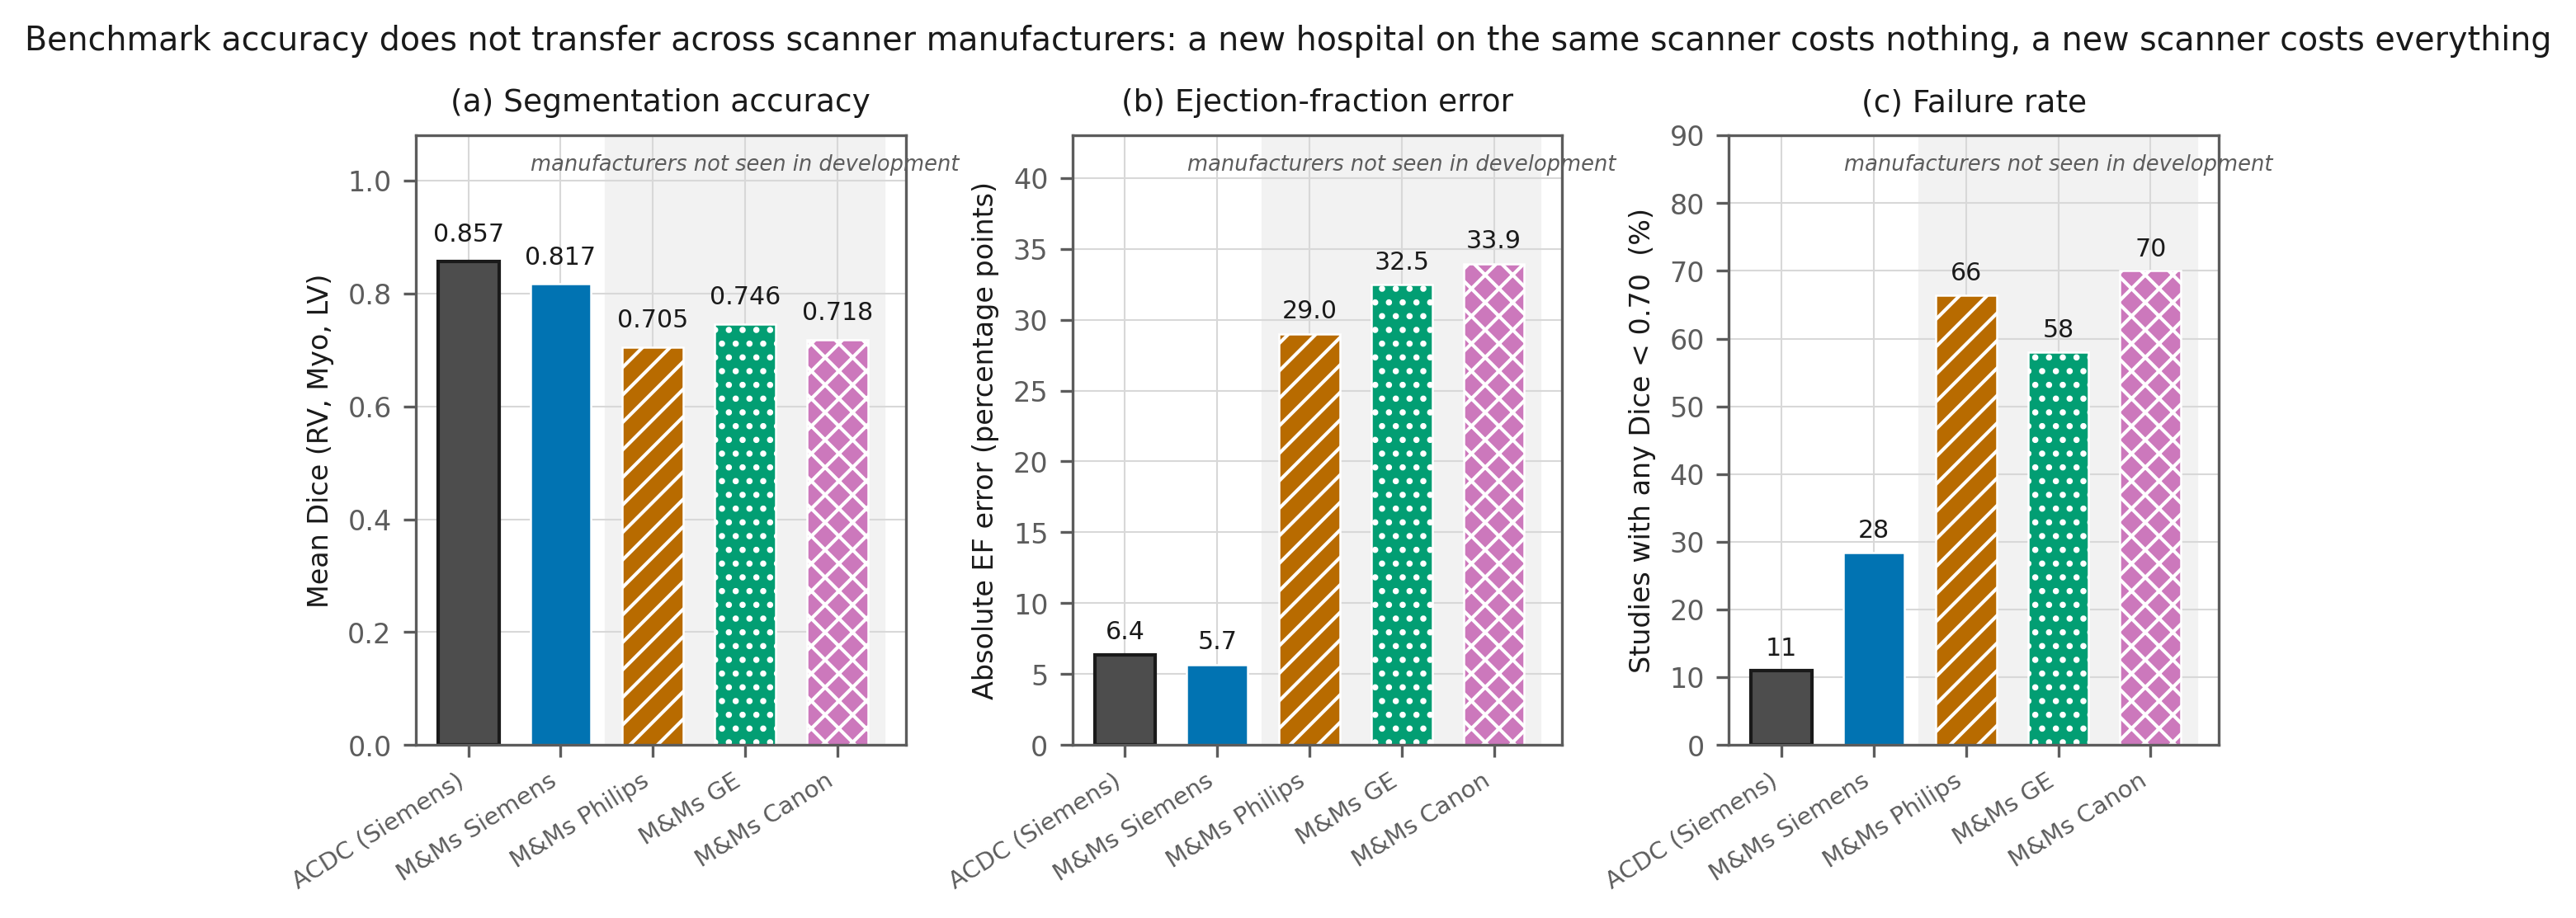
\includegraphics[width=\textwidth]{figures/fig1_vendor.png}
\caption{External validation on M\&Ms ($n=320$). ACDC is a single-vendor (Siemens)
benchmark. (a) Dice degrades modestly off-vendor. (b) Ejection-fraction error---the quantity
clinicians use---degrades sixfold. (c) The failure rate rises from 11\% to 70\% on Canon.}
\label{fig:vendor}
\end{figure}

\begin{figure}[t]
\centering
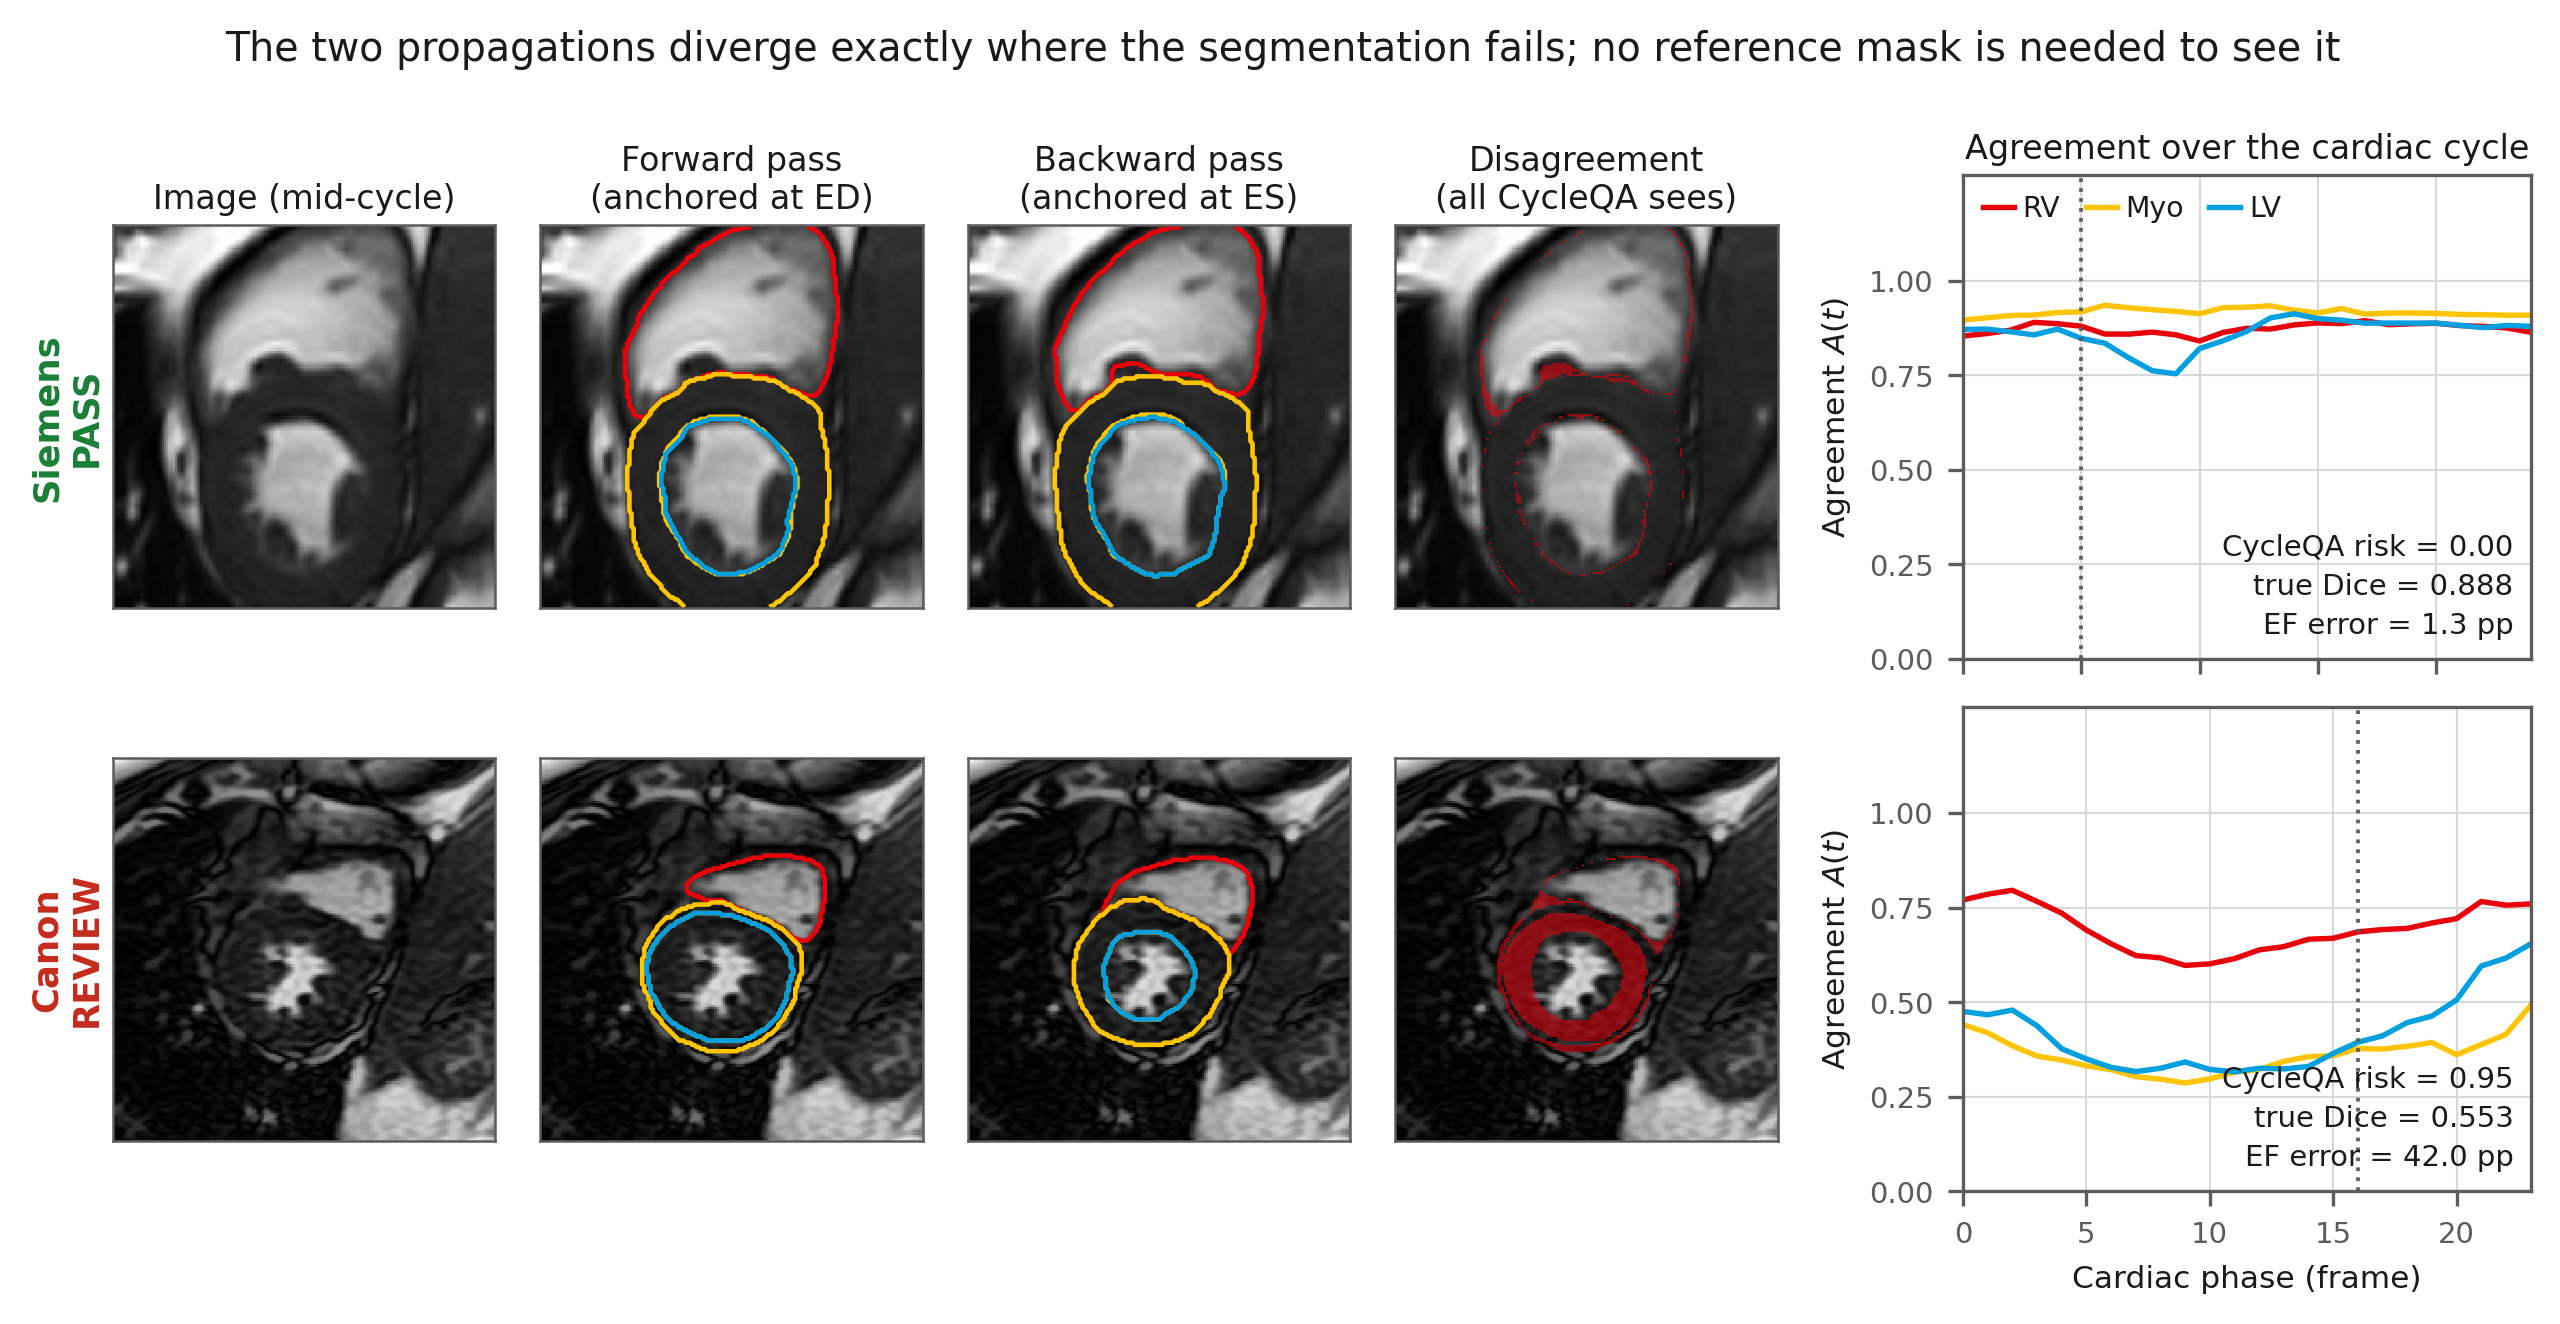
\includegraphics[width=\textwidth]{figures/fig2_qualitative.png}
\caption{The method, seen directly. Both rows show a mid-cycle frame, where \emph{neither}
propagation is anchored. \textbf{Top (Siemens, passed):} the forward and backward passes agree
almost everywhere; the disagreement map is a thin boundary rim, and $A(t)$ stays near 0.9.
\textbf{Bottom (Canon, flagged):} the two passes place the left ventricle and myocardium
differently, and the disagreement map is a large solid region---the model is contradicting itself.
$A(t)$ falls to 0.3--0.4. CycleQA assigns risks of 0.00 and 0.95 respectively. \textbf{Neither
judgement used a reference mask}: the fourth column is the only thing CycleQA is allowed to see.}
\label{fig:qual}
\end{figure}

\subsection{The failure is visible without ground truth}
Fig.~\ref{fig:qual} shows what this means on the images themselves. At a mid-cycle frame, where
neither propagation is anchored, a passing Siemens study has two passes that agree almost
everywhere, while a failing Canon study has two passes that place the ventricle and myocardium
differently---the disagreement map is a large solid region, and the model is visibly contradicting
itself. No reference mask is involved in producing that map.

Fig.~\ref{fig:est} and Table~\ref{tab:qc}(a) report Tier 1. Used \emph{directly}, with no
fitting of any kind, bidirectional disagreement estimates Dice with MAE 0.064 ($r=0.735$) on
ACDC and MAE 0.072 ($r=0.814$) on the external cohort. The signal is \emph{stronger} out of
domain than in it---it is most informative exactly where it is needed, because errors there
are larger and more varied.

\begin{figure}[t]
\centering
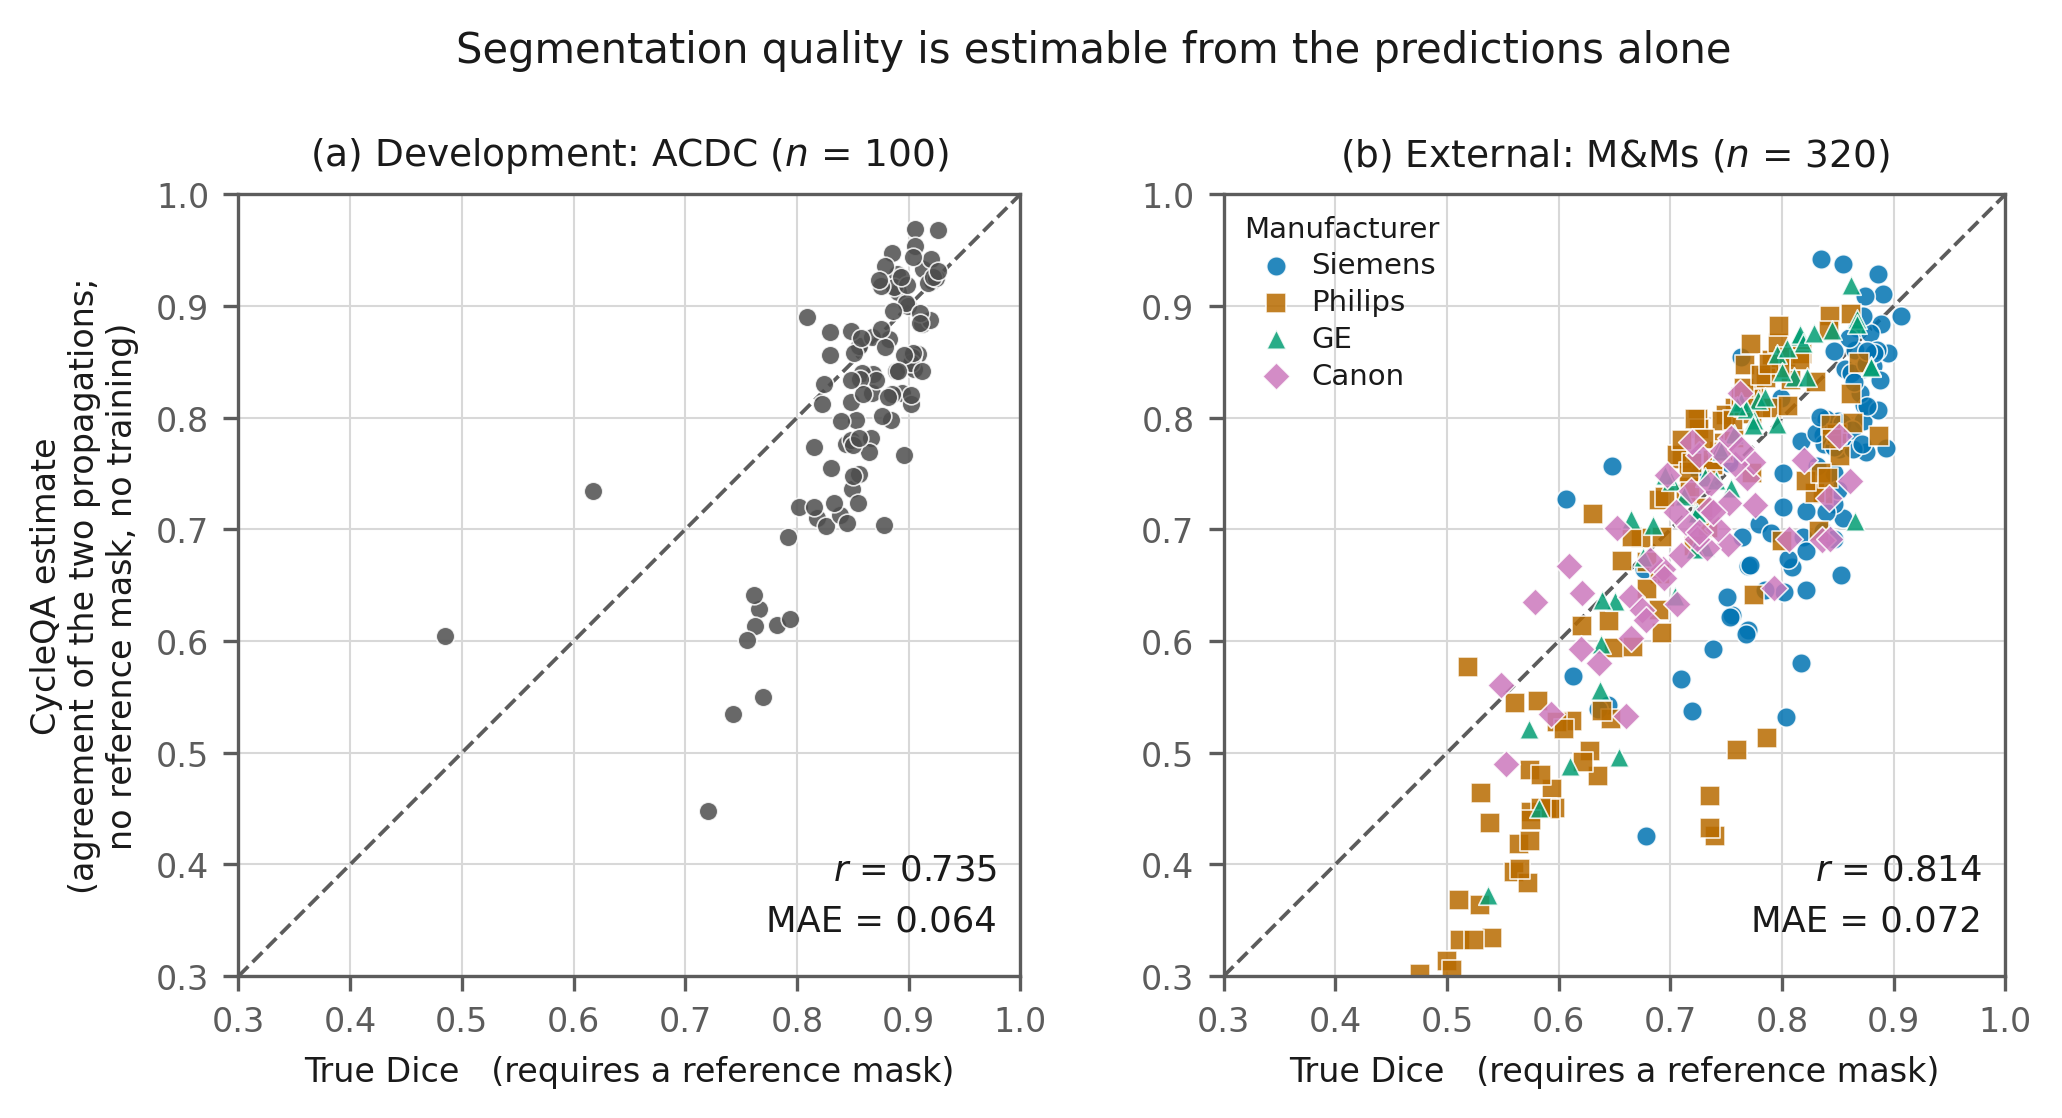
\includegraphics[width=\textwidth]{figures/fig3_estimation.png}
\caption{Segmentation quality is estimable without ground truth. The $x$-axis requires a
reference mask; the $y$-axis does not. No model is fitted.}
\label{fig:est}
\end{figure}

Table~\ref{tab:qc}(b) and Fig.~\ref{fig:det} report Tier 2. Frozen after development on
ACDC and applied once to M\&Ms, the risk model detects failed studies at AUROC 0.851
(0.810--0.892). Per vendor: Siemens 0.883, Philips 0.857, GE 0.823, \textbf{Canon 0.806}---a
manufacturer the model never saw. Calibration is reasonable (Brier 0.204) and the endpoint
is not fragile: sweeping the Dice threshold from 0.65 to 0.80 gives external AUROC 0.823 to
0.894, and the secondary EF endpoint gives 0.870.

The control (Fig.~\ref{fig:det}b) separates error detection from vendor detection. The
appearance-based detector reaches AUROC 0.478 for ``is this Canon?'' and 0.573 for ``is this
segmentation wrong?''---near chance at both. (Standard preprocessing---percentile clipping
and intensity normalisation---removes most of the raw appearance difference, yet the
segmentation still fails; the shift is not one that intensity statistics can see.)
\CQ{} reaches 0.636 and \textbf{0.851}. It is far better at finding the error than at
finding the vendor: it is an error detector, not a vendor classifier.

\begin{figure}[t]
\centering
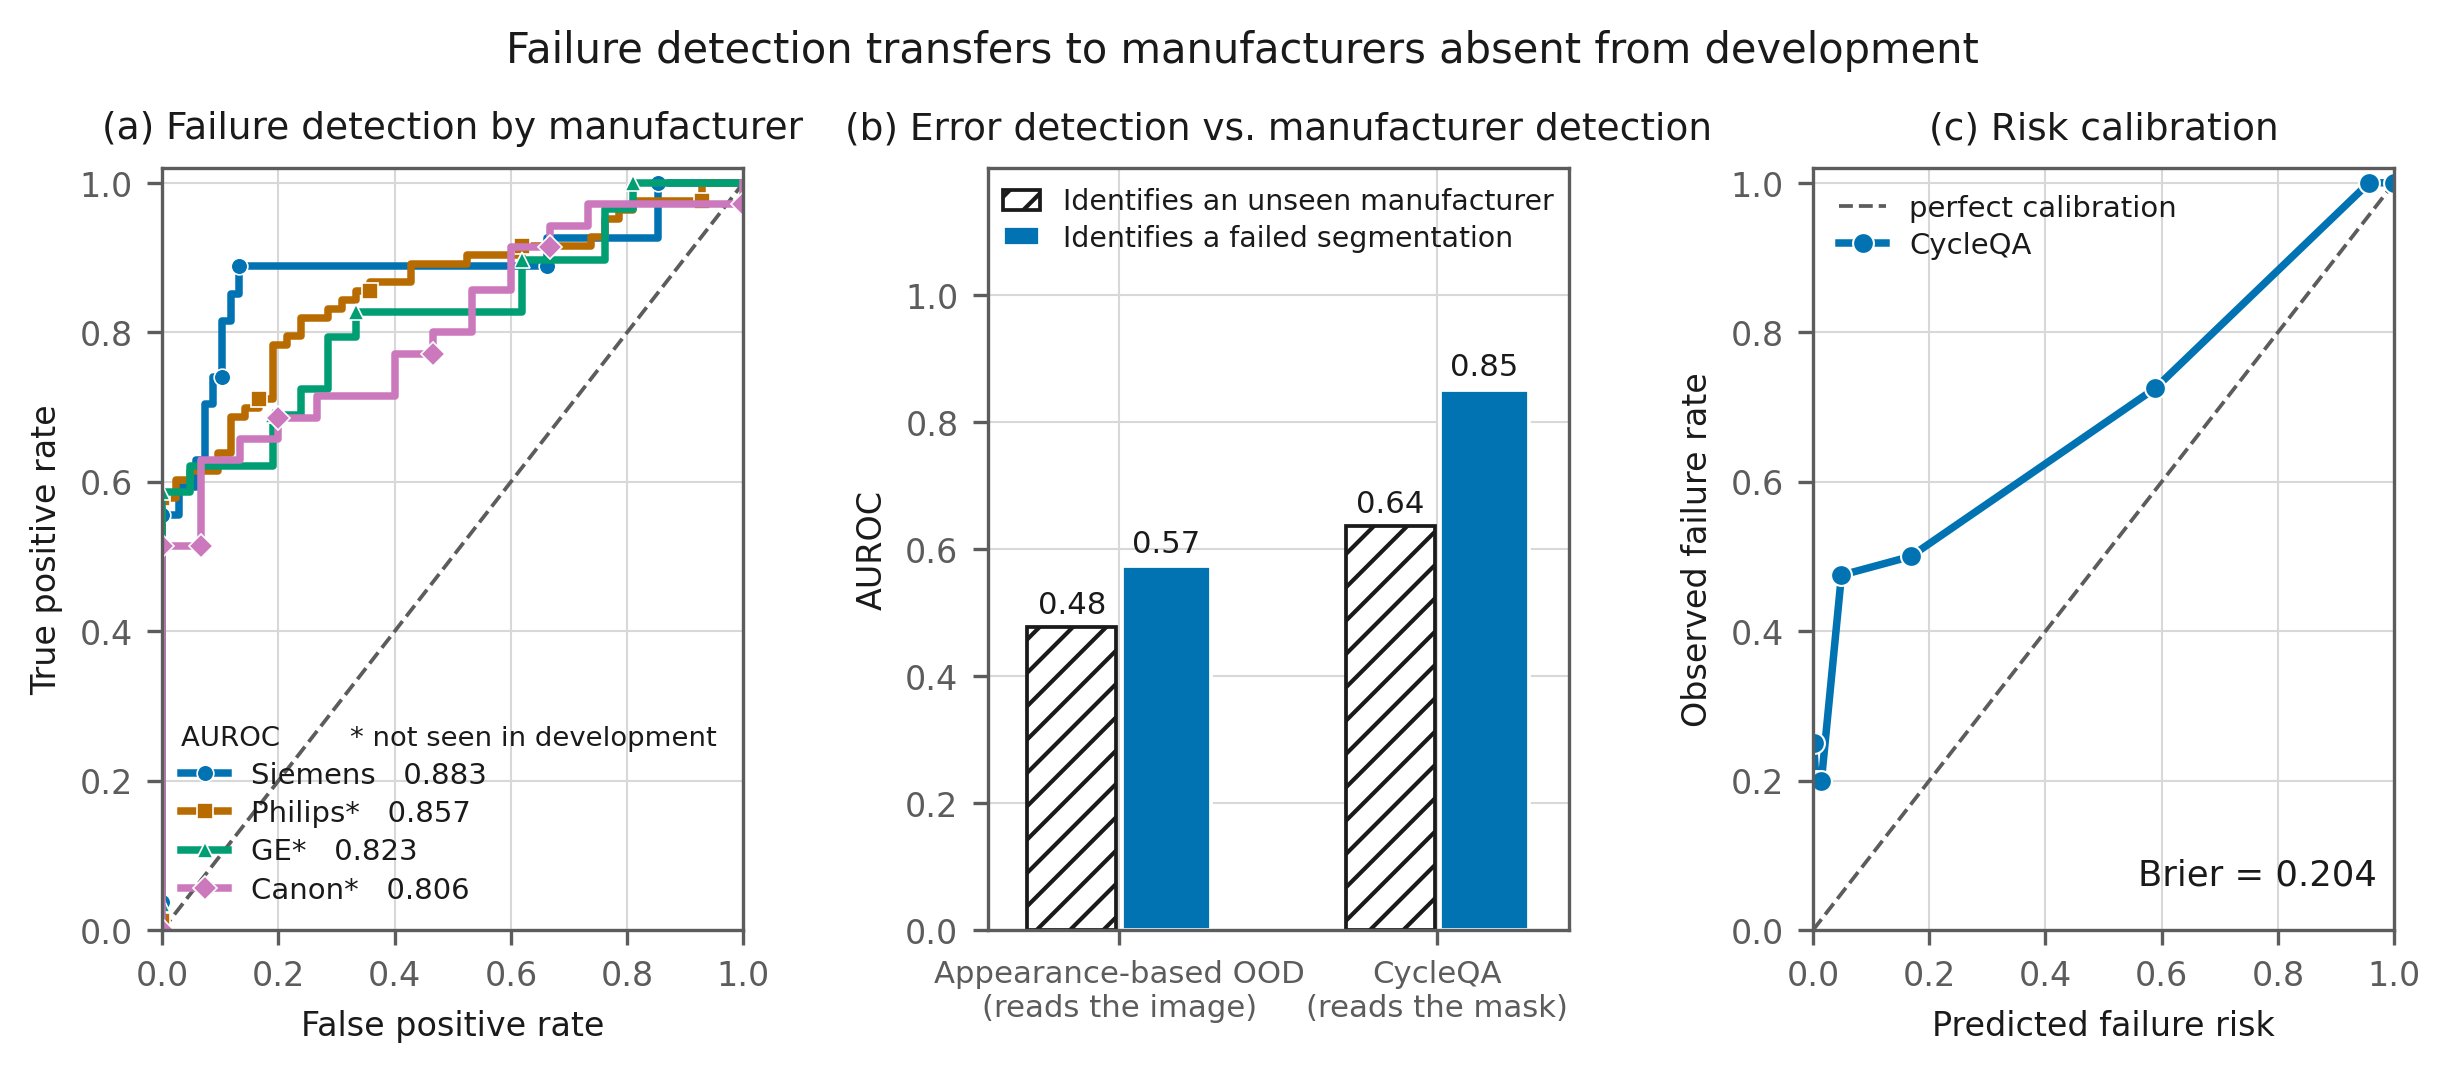
\includegraphics[width=\textwidth]{figures/fig4_detection.png}
\caption{Failure detection on M\&Ms. The risk model is frozen after ACDC and never sees
Philips, GE or Canon during development.}
\label{fig:det}
\end{figure}

\subsubsection{The ablation carries an honest surprise.}
Table~\ref{tab:qc}(c) is instructive. Anchor features alone reach an internal out-of-fold
AUROC of 0.987, but only 0.793 externally---the gap is a textbook signature of overfitting,
unsurprising when 24 features are fitted to 100 patients containing 11 failures. Yet the
\emph{untrained} rule---raw disagreement, no model at all---transfers at 0.850, better than
the learned anchor model. Plausibility features alone transfer best among learned models
(0.891). We therefore do not claim that learning is what makes \CQ{} work. The opposite is
true and is the more useful finding: \textbf{the disagreement signal is strong enough that
no training is required}, and on a development set of this size, training on it is actively
harmful.

\subsection{Acting on the risk score}
Fig.~\ref{fig:act} and Table~\ref{tab:qc}(d). Referring the highest-risk studies to human
review reduces residual error monotonically: reviewing the top 20\% lowers residual EF error
from 23.4 to 19.8 pp. This is real but modest---with a 54\% failure rate, a 20\% review
budget cannot fix much.

Reselection is far more effective, and costs nothing. The system already writes three
predictions per patient. Which is best is domain-dependent: on ACDC the merged output wins,
but on M\&Ms the ES-anchored propagation is markedly better (EF error 16.8 vs 23.4 pp)---a
fact one could only exploit with labels one does not have. Scoring each variant with \CQ{}
and keeping the most plausible reduces EF error to \textbf{12.0 pp} and the failure rate to
\textbf{14.7\%} (from 23.4 pp and 54.4\%), approaching the oracle (10.4 pp) and beating the
best fixed choice available only in hindsight (16.8 pp). No labels, no retraining, no
additional inference.

The per-vendor pattern reveals the mechanism. On Siemens, \CQ{} keeps the merged or
ED-anchored output (92\% of cases) and preserves an EF error of 5.8 pp---whereas
\emph{always} choosing ES, the best global strategy, would have wrecked it (14.8 pp). On
Canon, Philips and GE it switches predominantly to ES. \CQ{} adapts the anchoring strategy
per patient and per domain, without ever being told which vendor it is looking at.

\begin{figure}[t]
\centering
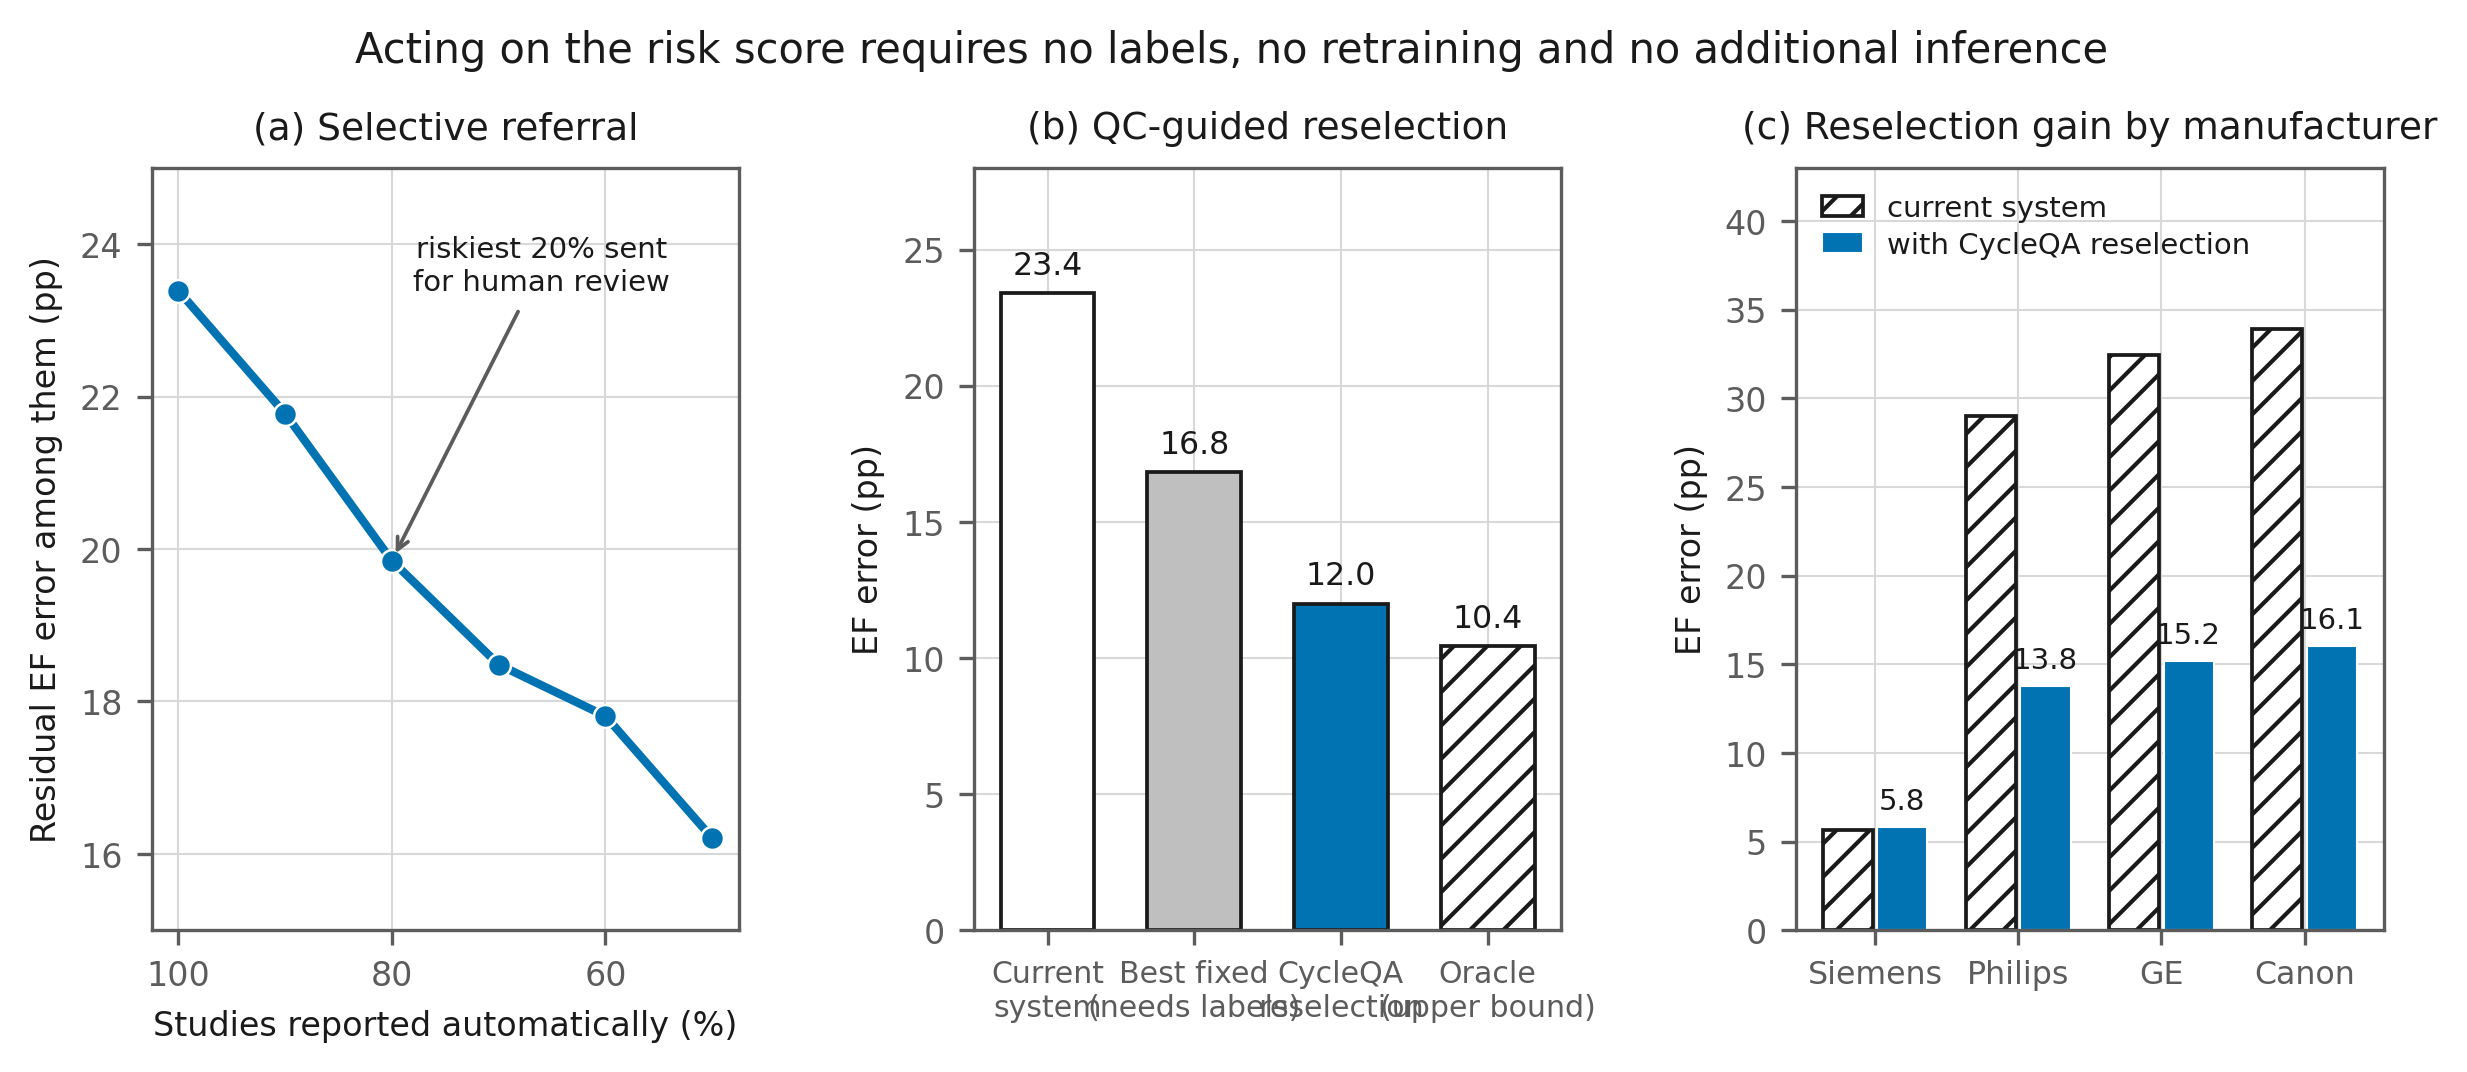
\includegraphics[width=\textwidth]{figures/fig5_action.png}
\caption{Acting on the risk score, M\&Ms ($n=320$). (b) The oracle selects the per-patient
minimum EF error and is an upper bound only for that quantity.}
\label{fig:act}
\end{figure}

\begin{table}[t]
\centering
\caption{The four families of \emph{no-reference} CycleQA features. Every quantity is computed from the predicted masks alone; none requires a reference mask, and none has access to the vendor, centre or pathology label. Anatomical and physiological constraints hold on any scanner \emph{by construction}, which is why the resulting detector transfers across vendors.}
\label{tab:features}
\setlength{\tabcolsep}{4pt}
\begin{tabular}{@{}p{2.5cm}p{3.9cm}p{4.6cm}c@{}}
\toprule
Family & Descriptors & Why it is vendor-invariant & $n$ \\
\midrule
Bidirectional agreement & $\overline{A}$, $\min A$, $A_{\mathrm{mid}}$, $\mathrm{sd}\,A$, $A_{10}$, decay, \% frames $A<0.7$ & Per frame $t$ and structure $c$, $A_c(t)=\mathrm{Dice}\!\left(M^{\mathrm{ED}}_t,M^{\mathrm{ES}}_t\right)$: the two independent propagations must converge if the model tracks the true anatomy. & 24 \\[2pt]
Anatomical plausibility & connected components; LV--myocardium containment; myocardial ring closure; LV holes; image-border contact & The myocardium must form a closed ring enclosing the LV cavity. Fragments, holes and border contact are anatomically impossible regardless of scanner. & 6 \\[2pt]
Temporal coherence & inter-frame IoU; LV centroid displacement; volume-curve roughness; cycle closure $|V(0)-V(T{-}1)|$; number of extrema of $V(t)$ & $V(t)$ must be smooth, periodic and close its cycle. Abrupt jumps or multiple minima indicate propagation drift. & 8 \\[2pt]
Physiological plausibility & $\mathrm{EDV}>\mathrm{ESV}$; EF within $[10,80]\%$; volume coefficient of variation; annotated ES frame is the volume minimum & Constraints on cardiac function that hold for every patient on every scanner. & 8 \\[2pt]
\midrule
\multicolumn{3}{@{}l}{Total} & 46 \\
\bottomrule
\end{tabular}
\end{table}

\begin{table}[t]
\centering
\caption{External validation of dual-anchored MedSAM2. ACDC is acquired on Siemens scanners only. Dice degrades modestly off-vendor, but the quantity clinicians actually use---ejection fraction---degrades by a factor of six, and the proportion of studies with a failed structure rises from 11\% to 70\%. Prompts are derived from the reference masks, so these are an \emph{oracle-prompt upper bound}.}
\label{tab:external}
\begin{tabular}{@{}lcccccc@{}}
\toprule
 & & \multicolumn{3}{c}{Dice} & EF error & Failure \\
\cmidrule(lr){3-5}
Cohort & $n$ & RV & Myo & LV & (pp) & (\%) \\
\midrule
\multicolumn{7}{@{}l}{\emph{Development (internal)}}\\
\quad ACDC (Siemens) & 100 & 0.913 & 0.801 & 0.858 & 6.4 & 11 \\
\midrule
\multicolumn{7}{@{}l}{\emph{M\&Ms (external)}}\\
\quad Siemens & 95 & 0.885 & 0.749 & 0.816 & 5.7 & 28 \\
\quad Philips$^{\dagger}$ & 125 & 0.743 & 0.674 & 0.697 & 29.0 & 66 \\
\quad GE$^{\dagger}$ & 50 & 0.768 & 0.729 & 0.742 & 32.5 & 58 \\
\quad Canon$^{\dagger}$ & 50 & 0.751 & 0.653 & 0.750 & 33.9 & 70 \\
\cmidrule(lr){1-7}
\quad All M\&Ms & 320 & 0.790 & 0.702 & 0.748 & 23.4 & 54 \\
\bottomrule
\end{tabular}

\smallskip
{\footnotesize $^{\dagger}$Vendor absent from the development set.}
\end{table}

\begin{table}[t]
\centering
\caption{CycleQA. \textbf{(a)} Bidirectional agreement used \emph{directly} as an estimate of Dice---no fitting of any kind. \textbf{(b)} Failure detection (any Dice $<0.70$); the risk model is developed on ACDC with patient-level nested 5-fold cross-validation, then \emph{frozen} and applied once to M\&Ms. \textbf{(c)} Feature ablation. \textbf{(d)} Acting on the risk score. Brackets are patient-level bootstrap 95\% CIs.}
\label{tab:qc}
\setlength{\tabcolsep}{5pt}
\begin{tabular}{@{}lccc@{}}
\toprule
\multicolumn{4}{@{}l}{\textbf{(a) Training-free Dice estimation}}\\
Cohort & $n$ & Pearson $r$ & MAE \\
\midrule
ACDC (internal) & 100 & 0.735 & 0.064 \\
M\&Ms (external) & 320 & 0.814 & 0.072 \\
\quad Siemens & 95 & 0.687 & 0.082 \\
\quad Philips & 125 & 0.862 & 0.083 \\
\quad GE & 50 & 0.911 & 0.045 \\
\quad Canon & 50 & 0.714 & 0.050 \\
\midrule
\multicolumn{4}{@{}l}{\textbf{(b) Failure detection: AUROC [95\% CI]}}\\
Method & \multicolumn{1}{c}{ACDC (out-of-fold)} & \multicolumn{2}{c}{M\&Ms (external)} \\
\midrule
Disagreement, no training & 0.909 & \multicolumn{2}{c}{0.850 [0.811, 0.888]} \\
Logistic regression & 0.915 & \multicolumn{2}{c}{0.851 [0.810, 0.892]} \\
Random forest & 0.900 & \multicolumn{2}{c}{0.853 [0.808, 0.892]} \\
\addlinespace
\quad Siemens & --- & \multicolumn{2}{c}{0.883 [0.780, 0.971]} \\
\quad Philips$^{\dagger}$ & --- & \multicolumn{2}{c}{0.857 [0.789, 0.915]} \\
\quad GE$^{\dagger}$ & --- & \multicolumn{2}{c}{0.823 [0.698, 0.923]} \\
\quad Canon$^{\dagger}$ & --- & \multicolumn{2}{c}{0.806 [0.675, 0.912]} \\
\midrule
\multicolumn{4}{@{}l}{\textbf{(c) Ablation: AUROC}}\\
Features & $n$ & ACDC (out-of-fold) & M\&Ms (external) \\
\midrule
anchor only & 24 & 0.987 & 0.793 \\
anat$+$temp$+$func (no anchor) & 22 & 0.863 & 0.891 \\
anchor $+$ anat & 30 & 0.979 & 0.789 \\
anchor $+$ anat $+$ temp & 38 & 0.959 & 0.804 \\
FULL (all four) & 46 & 0.915 & 0.851 \\
\midrule
\multicolumn{4}{@{}l}{\textbf{(d) Acting on the risk score (M\&Ms, $n=320$)}}\\
Strategy & Dice & EF error (pp) & Failure (\%) \\
\midrule
Current system (merged output) & 0.747 & 23.4 & 54.4 \\
Best fixed choice (hindsight) & 0.799 & 16.8 & 21.9 \\
\textbf{CycleQA reselection} & 0.815 & 12.0 & 14.7 \\
Oracle (minimum EF error) & 0.812 & 10.4 & 17.8 \\
\bottomrule
\end{tabular}

\smallskip
{\footnotesize $^{\dagger}$Vendor absent from the development set.}
\end{table}



\section{Discussion}

\subsubsection{Why quality assurance transfers when segmentation does not.}
The segmentation model must answer a hard question---\emph{which pixels are myocardium?}---and
to do so it must read appearance. Appearance is what changes between scanners, so the model
breaks. \CQ{} asks two easy questions: \emph{are you consistent with yourself?} and \emph{is
your answer anatomically possible?} Neither requires the image. A heart is a heart on any
scanner: the myocardium encloses the LV cavity, the volume curve closes, EDV exceeds ESV.
These constraints are vendor-invariant \emph{by construction}, which is why a detector built
on them survives a change of manufacturer that the segmenter does not. Verifying an answer
is easier than producing it---and so the watchdog is more robust than the model it watches.

\subsubsection{Deployment and post-market surveillance.}
A site installs the tool with no labels and no retraining. Every study receives a \CQ{} score
in about a second of CPU time, with no second network. Studies below threshold are
auto-reported; high-risk studies are flagged for review, with the risk--coverage curve
converting review capacity into a budgeted decision; and where a more plausible alternative
propagation exists, it is substituted automatically. Beyond the individual study, the
\emph{mean} \CQ{} risk across a site's workload is itself a label-free proxy for
performance: a drift above the development baseline is an alarm that the site is out of
distribution, raised before any patient has been misreported. Regulators require
post-market surveillance of deployed AI devices, and the usual obstacle is that the real
world supplies no ground truth. \CQ{} supplies a surrogate.

\subsubsection{Limitations.}
Prompts are derived from reference masks, so our numbers are an oracle-prompt upper bound;
real deployment additionally needs automatic prompt generation. Reference masks exist only
at ED and ES, so we validate annotated-phase error and make no claim about intermediate
phases. Evaluation is retrospective and on public data; there is no prospective clinical
validation. The review threshold is an operating choice each site must set against its own
risk tolerance. Finally, the development set (100 patients, 11 failures) is small---which is
precisely why the training-free tier, not the learned one, is our recommended configuration.
Supervised U-Net and DINOv2 baselines were also run on M\&Ms, but the provenance of their
training checkpoints could not be established with certainty, so they are excluded rather than
reported as a comparison that cannot be defended.


\section{Conclusion}

A zero-shot cardiac video foundation model that scores 0.91 Dice on a public benchmark
produces a 34-point ejection-fraction error on an unseen scanner---and at that site there is
no ground truth with which to notice. We showed the failure is legible from the predicted
masks alone, because dual-anchored propagation runs the same video twice and the two passes
disagree exactly when the model is wrong. Used without any training, that disagreement
estimates Dice to within 0.072 and detects failed studies at AUROC 0.850 on manufacturers
absent from development; used to reselect among predictions already computed, it halves
ejection-fraction error. The redundancy introduced to make the model accurate is the
redundancy that makes it self-auditing. A fragile model can be deployed safely if the
watchdog watching it is not fragile.


\subsubsection{Acknowledgements.} Removed for review.

\bibliographystyle{splncs04}
\bibliography{references}

\end{document}
